\chapter{Conceptual framework for translating NAPLAN scale scores into equivalent year levels} \label{chap1}

\section{The design of NAPLAN}

\subsection{NAPLAN scale scores}

Students that undertake the NAPLAN test receive a score for each assessment domain: reading, writing, language conventions (which includes spelling, grammar and punctuation), and numeracy. This score, called the NAPLAN scale score, is typically between 0 and 1000. While the scores are used to indicate whether a student is above NAPLAN national minimum standards for each year level, they have no other direct interpretation. The scores are an estimate of student skill level at a point in time, a latent concept -- the numbers themselves have no particular meaning.\footnote{It would be possible to link NAPLAN scale scores to curriculum standards, but this has not yet been developed. It is possible that NAPLAN scores will become more closely linked to curriculum standards with the move to NAPLAN online.} Nor are the scores comparable across assessment domains.

\subsection{Horizontal and vertical equating}

The NAPLAN test is designed so that results in each domain  can be compared between students in different year levels and students taking the test in different years. This means, for example, that a student who took the \mbox{Year 5} NAPLAN reading test in 2012 and received a scale score of 500 is estimated to be at the equivalent level of a student who took the \mbox{Year 7} reading test in 2013 and received the same score. That is, they are demonstrating comparable reading skills in the elements being tested by NAPLAN. This property of NAPLAN is achieved via a process known as \textit{horizontal} and \textit{vertical equating}.

The horizontal equating process involves a sample of students taking an equating test in addition to the NAPLAN tests. A scaling process takes place using this equating sample and common items across years on the equating tests. The result is that NAPLAN scale scores are comparable across different years. The vertical equating process involves common test items on the tests administered to different year levels. The results are scaled so that scale scores are comparable across different year levels.\footnote{See \textcite[][40--72]{acara2015a} for details.}

While the horizontal and vertical equating process is necessary to measure student progress over time, it also introduces an additional source of error into NAPLAN results.\footnote{See, for instance, \textcite{wu2010}.} The results presented in this analysis take the equating process as given, which means any errors arising from this process reduce the reliability of the analysis. We suggest that our analysis should be revisited after NAPLAN is moved online from 2017, as online testing is likely to strengthen the equating process.\footcite{acara2015b,wu2010}

\section{Looking at progress through a new lens}

\subsection{NAPLAN scale scores give an incomplete picture of student progress}

Student performance on standardised tests can be measured in a number of different ways.\footcite{angoff1984} The simplest measure, raw test scores, can be used to rank students. But raw scores can be hard to interpret. For example, on a 40-question test, the difference in skill level between a student with 25 correct answers and another with 20 correct answers should not be considered equal to the difference between a student with 40 correct answers and another with 35 correct answers. Raw test scores are even less useful for looking at student progress over time, because the measure does not take into account the degree of difficulty in the questions asked in different tests.

NAPLAN scale scores are developed from the Rasch model, an advanced psychometric model for estimating a student's skill level. The resulting estimates have a number of desirable properties, including being on an interval scale.\footnote{This means that, in terms of skill level on the construct being tested, the difference between a score of 400 and 450 is equivalent to the difference between 600 and 650, for example.} This property suggests that student progress can be measured by `gain scores': the difference between NAPLAN scale scores in two test-taking years.\footnote{NAPLAN is a test of specific literacy and numeracy skills. These skills are fundamental to student learning. Yet a standardised test does not cover all elements of student learning; for instance, NAPLAN tends to focus on specific skills rather than content knowledge. Thus, when the report refers to `learning' or `progress' in numeracy or reading, it is referring to that which can be measured by NAPLAN.} But there are limitations to using this measure, as ACARA notes: 
\textit{\begin{quote}
It is important to consider that students generally show greater gains in literacy and numeracy in the earlier years than in the later years of schooling, and that students who start with lower NAPLAN scores tend to make greater gains over time than those who start with higher NAPLAN scores.\footcite{acara2015c}
\end{quote}}

That is, the ``path of progress'' that students take across the four NAPLAN test years is not a linear function of the NAPLAN scale score, as shown in \Cref{fig:path}. Between 2012 and 2014 in numeracy, for instance, the median student made a gain of 86 points between Years 3 and 5 (an average of 43 points each year), 54 points between Years 5 and 7 (an average of 27 points each year), and 43 points between Years 7 and 9 (an average of 21.5 points each year).\footnote{Grattan analysis of \textcite{acara2014}.} 

ACARA implicitly acknowledges this non-linear growth path in the way that NAPLAN proficiency bands are defined. Specifically, the national minimum standard jumps by two bands from \mbox{Year 3} to \mbox{Year 5}, but only one band from \mbox{Year 5} to \mbox{Year 7} and from \mbox{Year 7} to \mbox{Year 9} (see \Vref{box:proficiency_bands}). Even so, proficiency bands do not adequately take non-linearity into account and so we do not use them in the \textit{Widening gaps} report.

Given that the observed growth in NAPLAN scores is not-linear with student year level, what does this mean? One interpretation would be to say that the education system is less effective for students in later year levels, especially between \mbox{Year 7} and \mbox{Year 9}. This would be an important finding.

Of course, it could be that the smaller gain scores observed between higher year levels can be attributed to teaching differences -- for instance, a shift from skill development to content knowledge in secondary school. But if this was the case, we would expect gain scores to be strongly related to year level, and only weakly related to prior test score once year level is taken into account. \Vref{fig:gain_prior} suggests that this is not the case: lower prior scores are associated with higher gain scores \textit{within} each year level, and the same pattern holds for different population sub-groups.\footnote{Year level appears to have some effect, particularly for numeracy, but the impact is relatively weak once prior scores are taken into account.}
\begin{figure}[t]
 \captionwithunits{The relationship between NAPLAN scale scores and year level is not linear for the median student}{NAPLAN scale score of median student in each year level, Australia}
 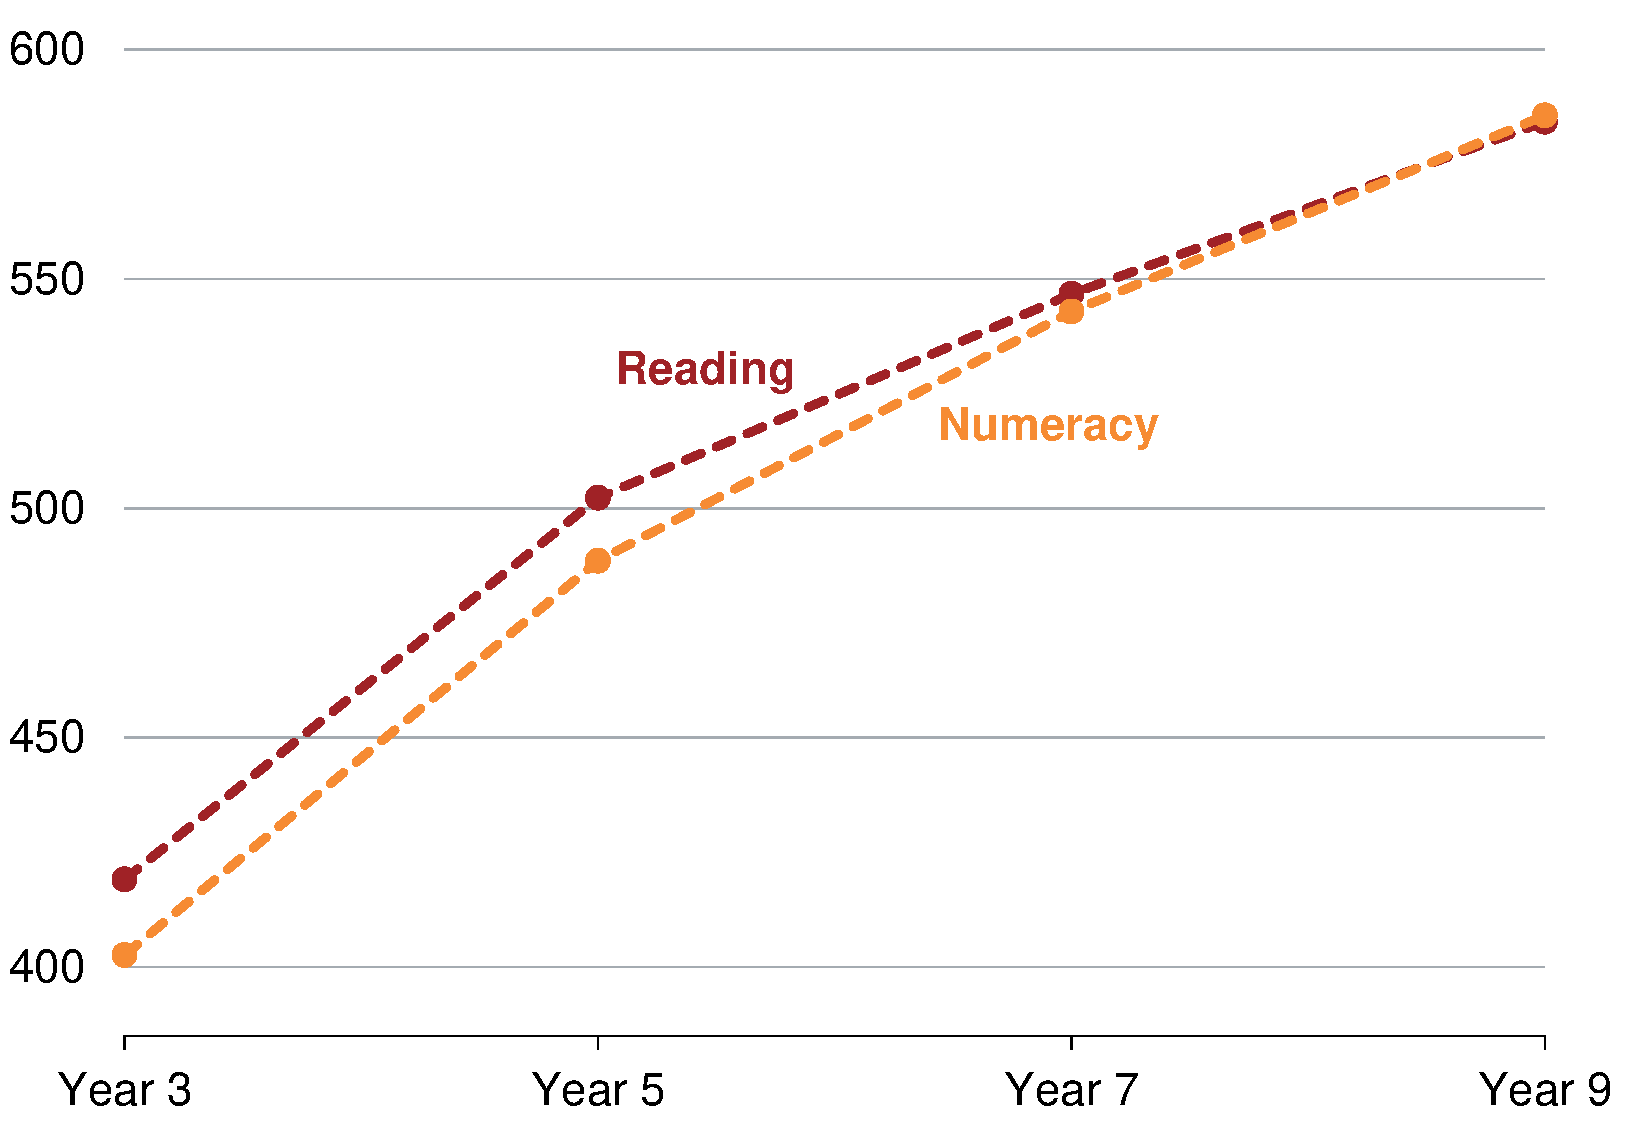
\includegraphics[width=\columnwidth]{atlas/PoP.pdf}\label{fig:path}
 \notes{Based on 2014 and 2012 median scores.}

\source{Grattan analysis of \textcite{acara2014}.}
\end{figure}

\begin{figure}[t]
 \captionwithunits{Higher gain scores are observed for lower prior scores, regardless of year level or population sub-group}{Median NAPLAN gain score over two years by prior score, 2014, Australia}
 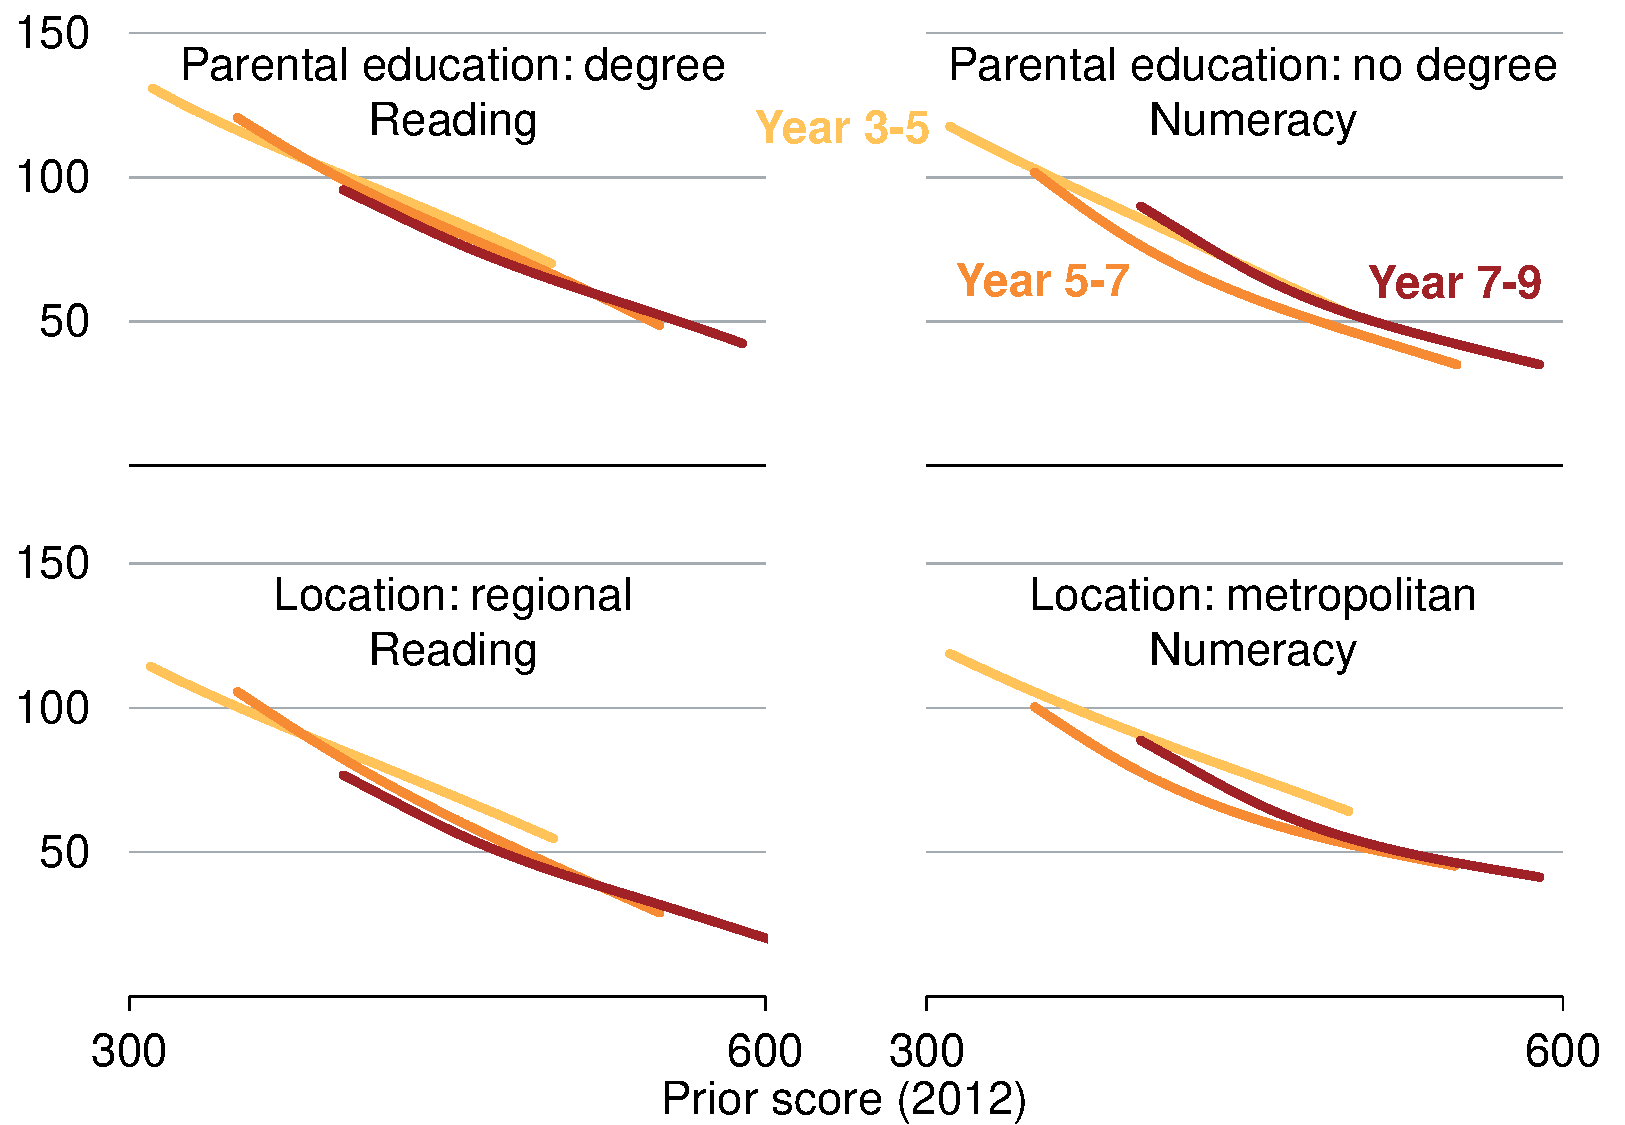
\includegraphics[width=\columnwidth]{atlas/Gain_prior.pdf}\label{fig:gain_prior}
\notes{Similar patterns exist for other sub-groups, and at different percentiles. Gain scores estimated by a median quantile regression with cubic regression splines.}

\source{Grattan analysis of \textcite{acara2014}.}
\end{figure}

A third interpretation is that students genuinely increase their skill level faster from a lower base, and slow down over time. That is, the higher a student's current skill level, the longer it takes to increase their skill level by a given amount (as measured by the NAPLAN scale). This appears to be the favoured interpretation among psychometricians.

Regardless of the explanation, this pattern of higher gain scores from lower starting scores should be taken into account when comparing the relative progress of different sub-groups of students. If not, it is too easy to draw spurious conclusions about the progress of different groups by over-interpreting gaps or gains in NAPLAN scores to mean something about broader learning progress.


\begin{bigbox*}{NAPLAN proficiency bands do not adequately take non-linearity into account}{box:proficiency_bands}
\raggedright

ACARA implicitly acknowledge the non-linear path of progress in the way that results are reported against \textit{NAPLAN proficiency bands}. There are ten proficiency bands spanning \mbox{Year 3} to \mbox{Year 9}, with equally-spaced cut-points along the NAPLAN scale.\footnote{With the exception of Band 1 and Band 10, each band spans 52 NAPLAN scale points.} These bands are used to define the National Minimum Standards. But because student skill level does not increase linearly over time, the National Minimum Standard increases by two bands between Years 3 and 5, but by only one band between Years 5 and 7 and between Years 7 and 9.\footnote{The National Minimum Standard is Band 2 for \mbox{Year 3}, Band 4 for \mbox{Year 5}, Band 5 for \mbox{Year 7}, and Band 6 for \mbox{Year 9}.} If there was reason to believe that the path of progress should be linear, then the change in the National Minimum Standards between each year level should be consistent. 

Six proficiency bands are reported for each year level. For a student to remain in the same \textit{relative} proficiency band, they must move up two bands between Years 3 and 5, then one band between Years 5 and 7, and another band between Years 7 and 9. But students who remain in the same relative band have not necessarily been progressing at the same rate.

\Cref{fig:npb} provides an example of this -- Student A moves from Band 4 in \mbox{Year 3} to Band 6 in \mbox{Year 5}, staying two bands above the national minimum standard. Student B performs consistently in the national minimum standard band, moving from Band 4 in \mbox{Year 5} to Band 6 in \mbox{Year 9}. Both students remain in the same

\begin{figure}[H]

 \captionwithunits{The level of growth required to remain in the same relative proficiency band changes with year level}{NAPLAN proficiency band}
 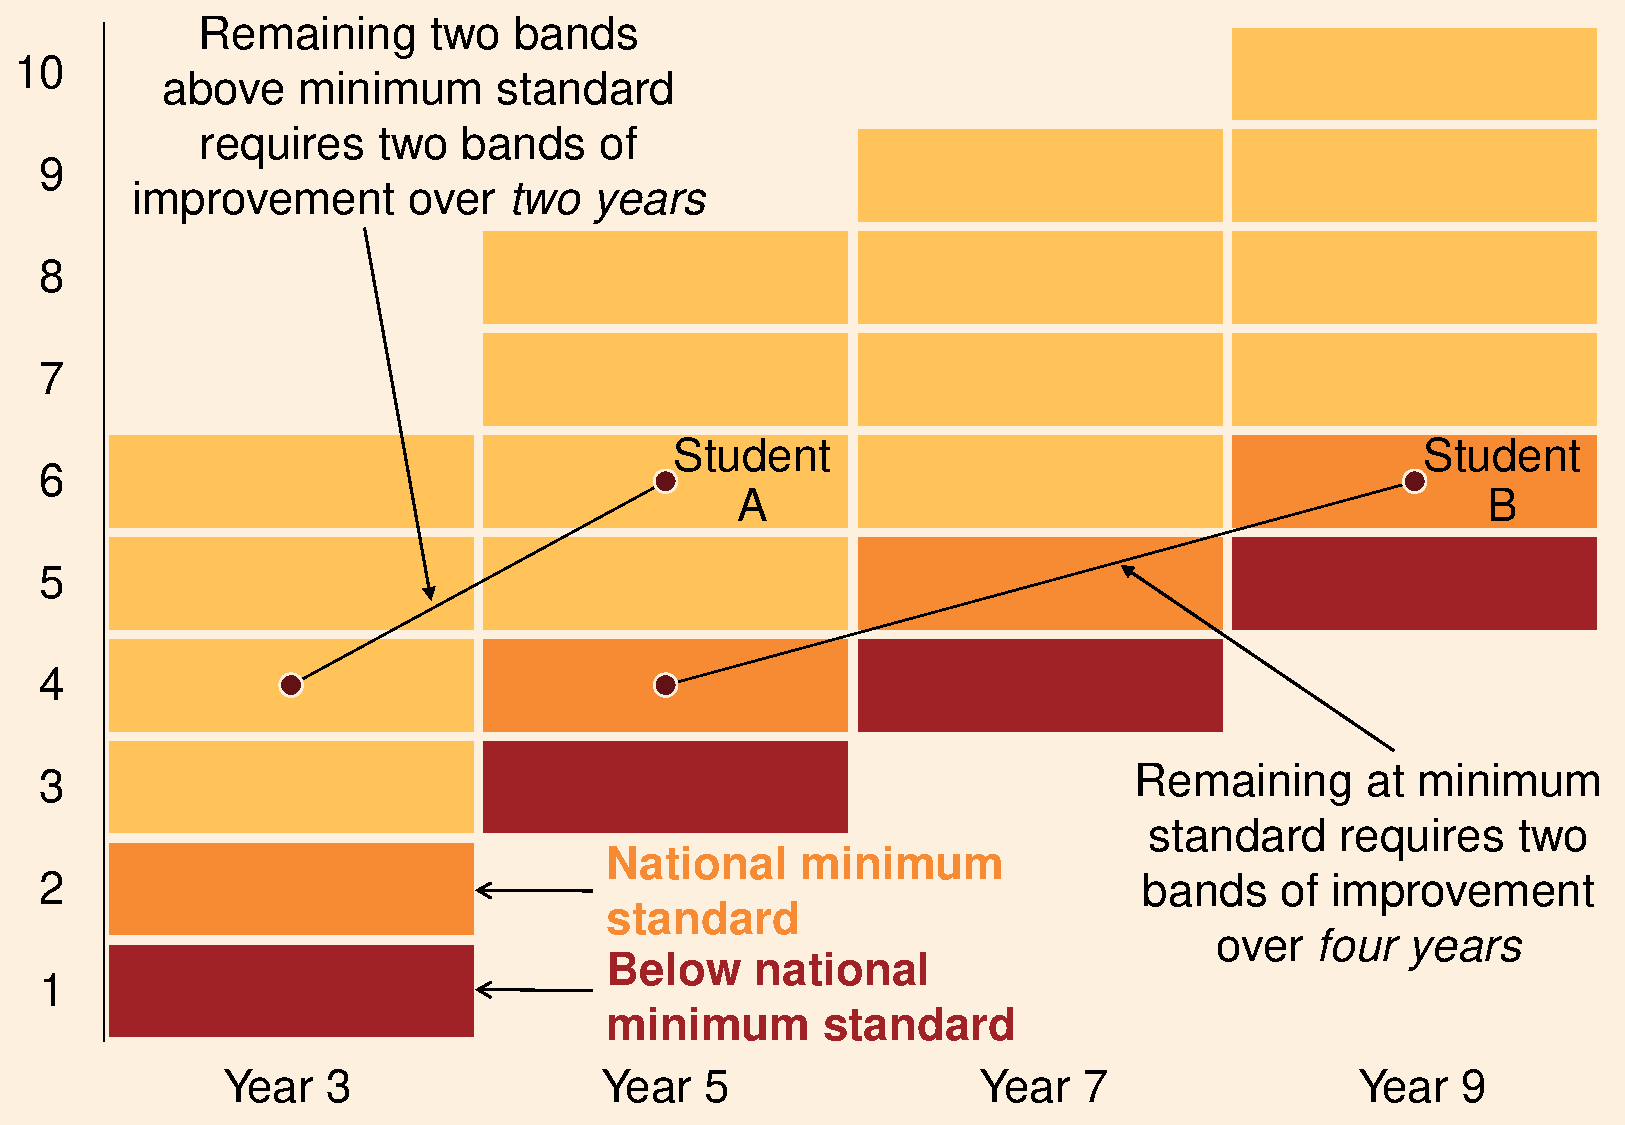
\includegraphics[width=\columnwidth]{atlas/NPB.pdf}\label{fig:npb}

\source{\textcite{acara2015a}.}
\end{figure}
\vspace{-10pt}

relative proficiency band, which suggests they are learning at the same rate. Yet Student A makes the same gain over two years as Student B does over four. This suggests that the non-linear scale of proficiency bands does not consistently account for the non-linear path of progress for students at different skill levels.\footnote{The analysis in this report does not use NAPLAN proficiency bands to assess student progress.}  

\end{bigbox*}

For example, students from remote areas score below students from metropolitan areas in \mbox{Year 3}, yet make higher gain scores, on average.\footnote{See also Figure 2 and Section 1.5 in the main \textit{Widening gaps} report, \textcite{goss2016}.} That is, remote children are increasing their skill level, as measured by NAPLAN, by more than metropolitan children. But it would be incorrect to infer from this that the remote students are catching up to metropolitan students in a broader sense. To catch up, a student who is behind must at some stage learn faster (comparing the rates of learning over the same set of skills). In fact, when we compare the gain scores of remote and metropolitan students \textit{from the same score in \mbox{Year 3}}, students from remote areas consistently make lower gain scores (at the median) than those from metropolitan areas, as shown for reading in \Cref{fig:remote_metro}. Remote students are actually falling further behind metropolitan students. 

Some researchers have accounted for the non-linearity in the student path of progress using `like-for-like' comparisons. That is, they have only compared gain scores across different sub-groups from the same prior score.\footnote{This type of analysis could also be performed for students that have the same end score.} Like-for-like comparisons can be useful for interpreting gains made by different sub-groups, as the example with metropolitan and remote students shows. But this approach is limited in its scope -- many population sub-groups start from very different skill levels. To compare the relative progress of students starting from different skill levels requires a new lens.

\begin{figure}[H]
 \captionwithunits{Remote students make higher gains on average  than metropolitan students, but lower gains from the same starting score}{Median NAPLAN gain score between \mbox{Year 3} (2012) and \mbox{Year 5} (2014), reading, Australia}
 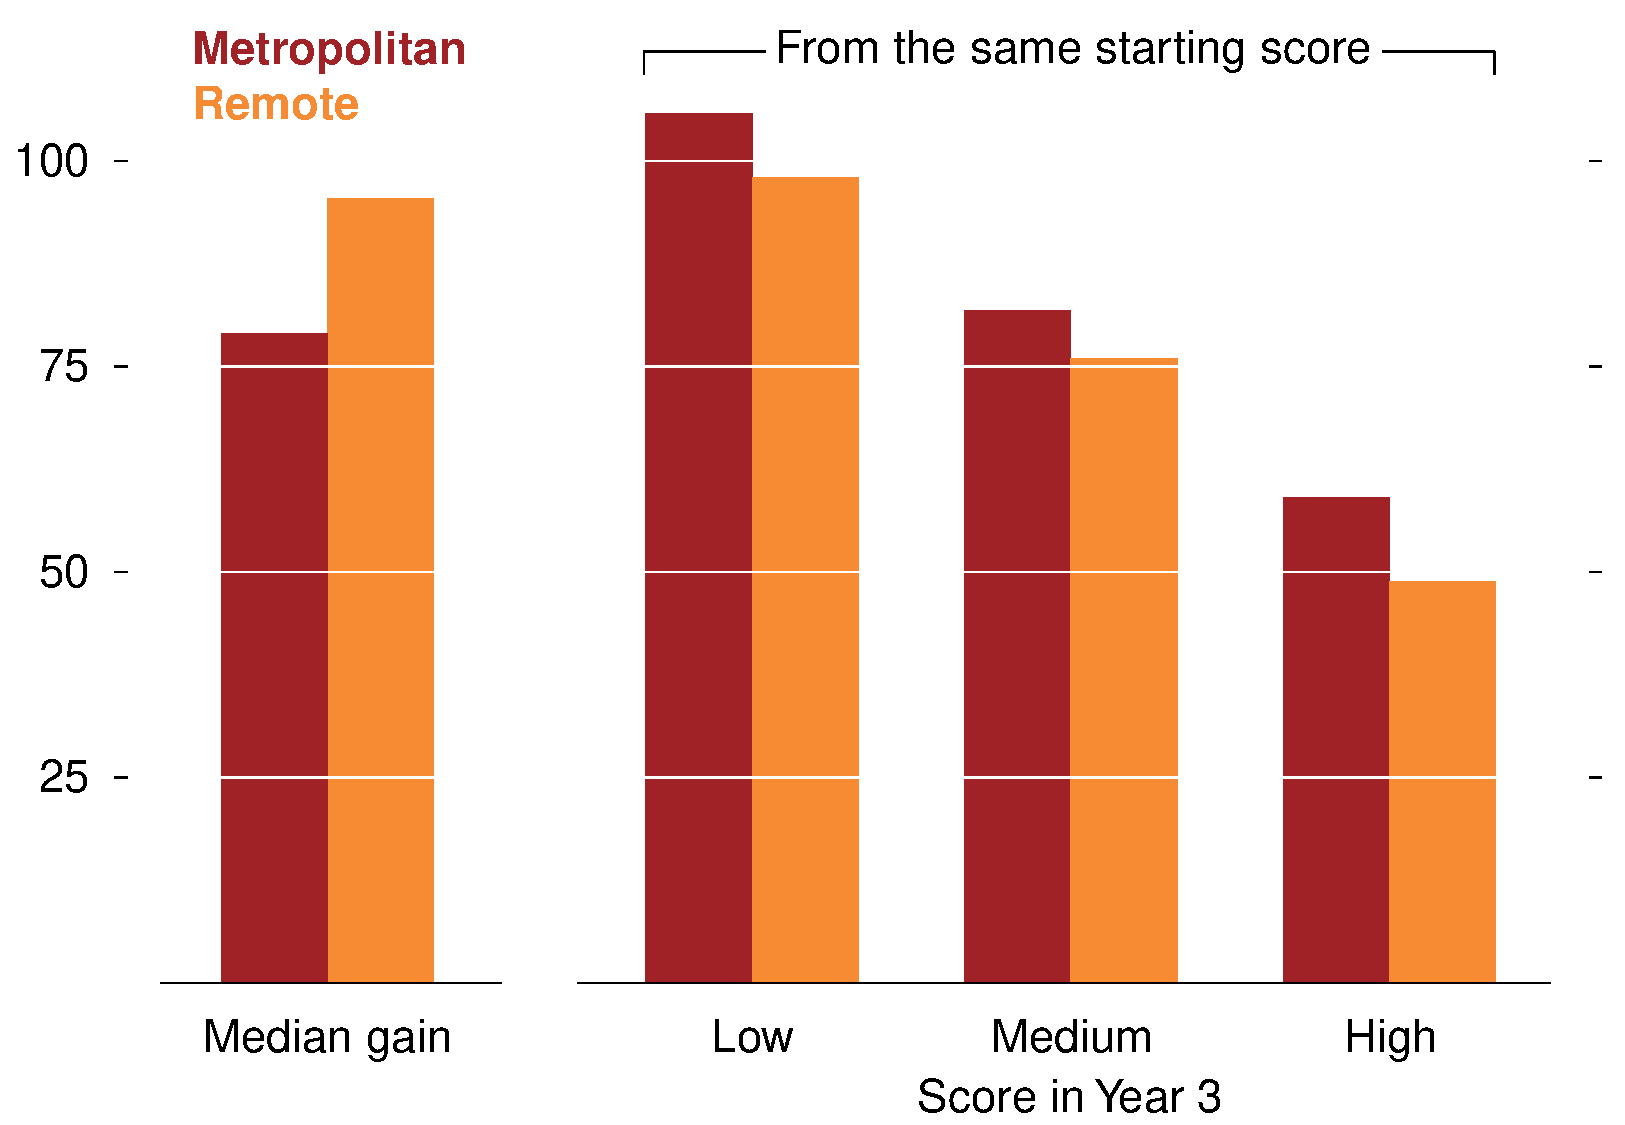
\includegraphics[width=\columnwidth]{atlas/remote_metro.pdf}\label{fig:remote_metro}
\notes{'Low, medium and high' \mbox{Year 3} scores are defined as the 20th, 50th, and 80th percentiles respectively. A similar pattern between metropolitan and remote students exists for numeracy.}

\source{Grattan analysis of \textcite{acara2014}.}
\end{figure}

\newpage

\subsection{Looking at progress through the lens of time}

An alternative measure of student progress is to define a \textit{year of progress} as the improvement expected from a typical student over a year. This measure would take into account that the typical student makes smaller gains in NAPLAN scale scores as they move further up the NAPLAN scale. That is, the NAPLAN gain score required for the typical student to make two \textit{years of progress} (in terms of the literacy and numeracy skills tested by NAPLAN) between Years 5 and 7 would be smaller than that required between Years 3 and 5.

\textit{Years of progress} is a measure of student progress relative to their peers, rather than a measure of their absolute \textit{skill level}. This measure gives NAPLAN results new meaning. It can also suggest a very different interpretation of what is happening compared to a `face value' intrepretation of gain scores or gaps in NAPLAN scale scores.\footnote{In longitudinal comparisons of two groups of students, changes over time in gaps between the groups are directly related to differences in gain scores.}
Consider two distinct groups of students: Group A and Group B. The scores displayed on \Cref{fig:example} are those of a representative student within each group (the median student): call these students A and B. Student A scores close to the average for numeracy, while Student B is below average, 103 NAPLAN points behind Student A in \mbox{Year 3}. Looked at in terms of NAPLAN points, as shown on the left chart, the gap between the students has reduced from 103 points in \mbox{Year 3} to 71 points in \mbox{Year 9}.\footnote{This does not account for within-group variation, but it suggests the typical student in Group B is catching up to the typical Student in Group A: Student B has a larger gain score between \mbox{Year 3} and \mbox{Year 9} than Student A.} At face-value, this suggests that Group B are catching up to Group A.

\begin{figure}[H]
 \captionwithunits{Measuring progress in years suggests a very different interpretation of NAPLAN results}{NAPLAN scale score}
 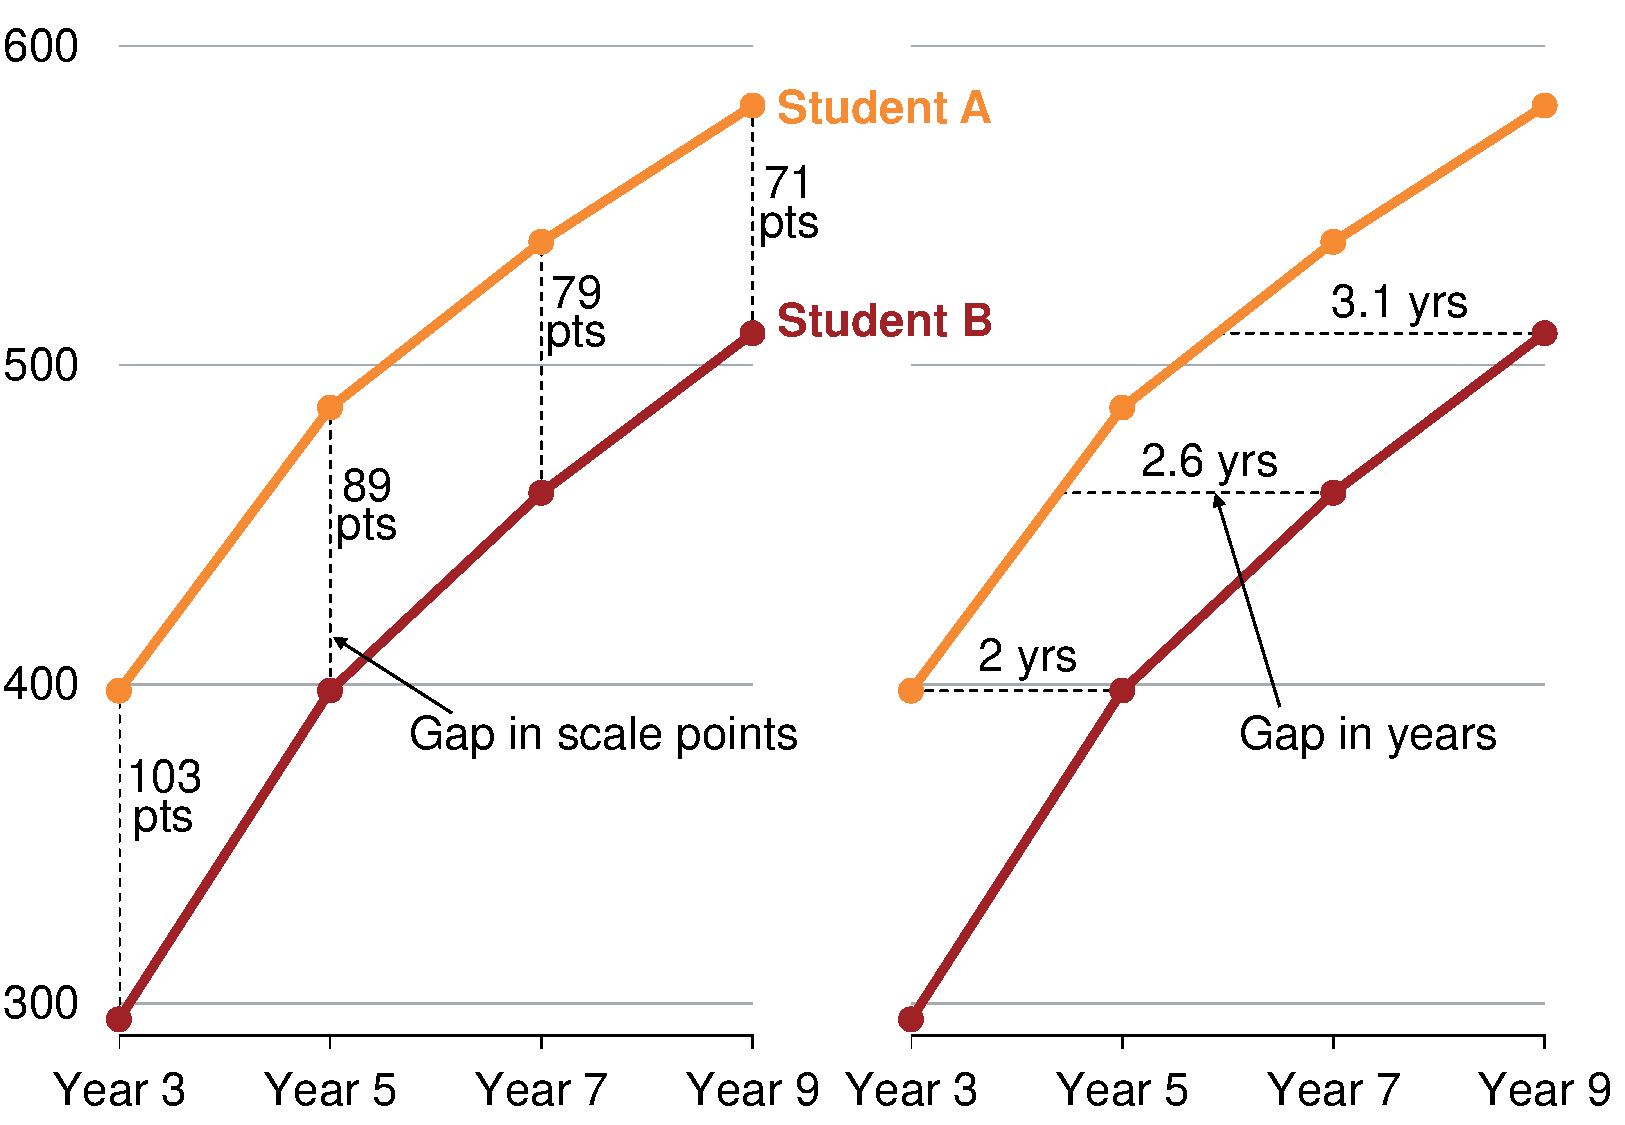
\includegraphics[width=\columnwidth]{atlas/NSSvsY.pdf}\label{fig:example}
\notes{The data in the charts is hypothetical, but the points on both charts are identical.}

\source{Grattan analysis.}
\end{figure}
\vspace{-6pt}

Yet the chart on the right tells a different story. In \mbox{Year 5}, Student B is performing at the level of Student A in \mbox{Year 3}. But by the time they reach \mbox{Year 9}, Student B's score is roughly half way between Student A's scores in \mbox{Year 5} and \mbox{Year 7}: Student B is performing at about the level of Student A in Year 6. This suggests that Group B has made about one \textit{less} year of progress than Group A between Years 5 and 9. Looking at progress through the lens of time suggests that Group B are falling further behind, not catching up.

\newpage
\section{Measuring \textit{Years of Progress}}

If we interpret the difference between students A and B according to the chart on the right of \Cref{fig:example}, then Student B makes roughly the same progress over four years (between \mbox{Year 5} and \mbox{Year 9}) as Student A makes in three years (between \mbox{Year 3} and Year 6). The difference between the students is defined in terms of Student A's rate of learning, but it could just as easily be defined in terms of Student B's rate of learning: ``how long will it take Student B to reach the level of Student A?''. While the story -- that Student A learns comparable skills in less time than Student B -- remains the same regardless of which student is defined as the benchmark, the size of the gap between the two in terms of `years and months' is different. In \mbox{Year 5}, for instance, Student B is performing at Student A's level two years earlier, but Student B will take about three years to reach Student A's current level. We could say that Student A is two years ahead, but we could also say that Student B is three years behind. To compare progress in terms of years and months across different groups requires a common benchmark. 

If NAPLAN scores were linked to absolute curriculum standards that define the expected capabilities for each year level, this would provide a common benchmark for measuring progress in terms of time. But given such standards have not been developed, we define a relative benchmark instead.

The results presented in \textit{Widening gaps} use the median or `typical' student's results as a benchmark for comparing other groups of students. That is, a year of progress is defined according to the gain score expected from the median student at a given level if they were to take the NAPLAN test today and again in one year's time.\footnote{Because NAPLAN is taken every two years, it is only possible to observe gain scores over two-year periods. But it is straightforward to interpolate this for a single year of progress.}

NAPLAN scale scores are mapped onto the path of progress of the typical student across their schooling years. We define the schooling year associated with each NAPLAN score as an \textit{equivalent year level}. This type of measure is not new. For instance, the \textit{Programme for International Student Assessment} (PISA) reports a relative grade measure to compare students within each country.\footcite{oecd2013} Grade equivalent scales have also been used in reporting results of other standardised tests.\footnote{See, for instance, \textcite{renaissance2015}.}

It is straightforward to estimate the score corresponding to equivalent year levels 3, 5, 7, and 9; these are the observed median scores for each test-taking year. In \mbox{Year 5} numeracy in 2014, for instance, the median NAPLAN scale score is approximately 489. A student with a score of 489 in any test-taking year is said to be performing at equivalent year level 5 (using 2014 as a reference year), meaning that their numeracy skill level is the same as a typical \mbox{Year 5} student.

To estimate the median NAPLAN scale score for year levels between \mbox{Year 3} and \mbox{Year 9}, we fit a curve through the estimated points for Years 3, 5, 7 and 9. This assumes that median student learning follows a smooth trajectory, as opposed to coming in short bursts.\footnote{This might not be the case for an individual student, but it is a reasonable assumption for the median of a large group of students.}

\newpage
To estimate the median NAPLAN scale score below \mbox{Year 3} or above \mbox{Year 9} is more challenging. Without data on \mbox{Year 2} students, for instance, it is difficult to estimate the skill level of a typical \mbox{Year 2} student in terms of the NAPLAN scale. But linked data -- for instance, \mbox{Year 3} results in 2012 linked to \mbox{Year 5} results in 2014 -- can be used to estimate the relationship between the \mbox{Year 3} score and the two-year gain score. Some students will have scored at about the level of a typical \mbox{Year 4} student on the \mbox{Year 5} test, meaning they are estimated to be one year behind the typical \mbox{Year 5} student. We assume that these students were, on average, one year behind the typical \mbox{Year 3} student when they were in \mbox{Year 3}. Similarly, using \mbox{Year 7} results linked to \mbox{Year 9} results, we assume that students who are two years ahead in \mbox{Year 7} are two years ahead in \mbox{Year 9}, on average. 

Using a regression approach, we estimate the median NAPLAN scale score for students who are as much as 18 months behind in \mbox{Year 3} (which we refer to as equivalent year level 1.5, or Year 1 and 6 months), and as far as 24 months ahead in \mbox{Year 9} (which we refer to as equivalent year level 11).\footnote{It is important to emphasise that this approach is based on data from below-average students in \mbox{Year 3} and above-average students in \mbox{Year 9}; it is not an extrapolation of the curve constructed between \mbox{Year 3} and \mbox{Year 9}.} It is possible to extrapolate the curve further than two years ahead of \mbox{Year 9}, but the results are less robust at such points. \Cref{fig:cyl_n} shows conceptually how these approaches are used to construct a curve that maps NAPLAN scale scores to estimated equivalent year levels. The methodology is described in more detail in \Cref{chap3}.

\begin{figure}[H]
 \captionwithunits{Estimating the equivalent year level benchmark curve involves interpolation and regression}{Estimated median NAPLAN scale score, numeracy, Australia}
 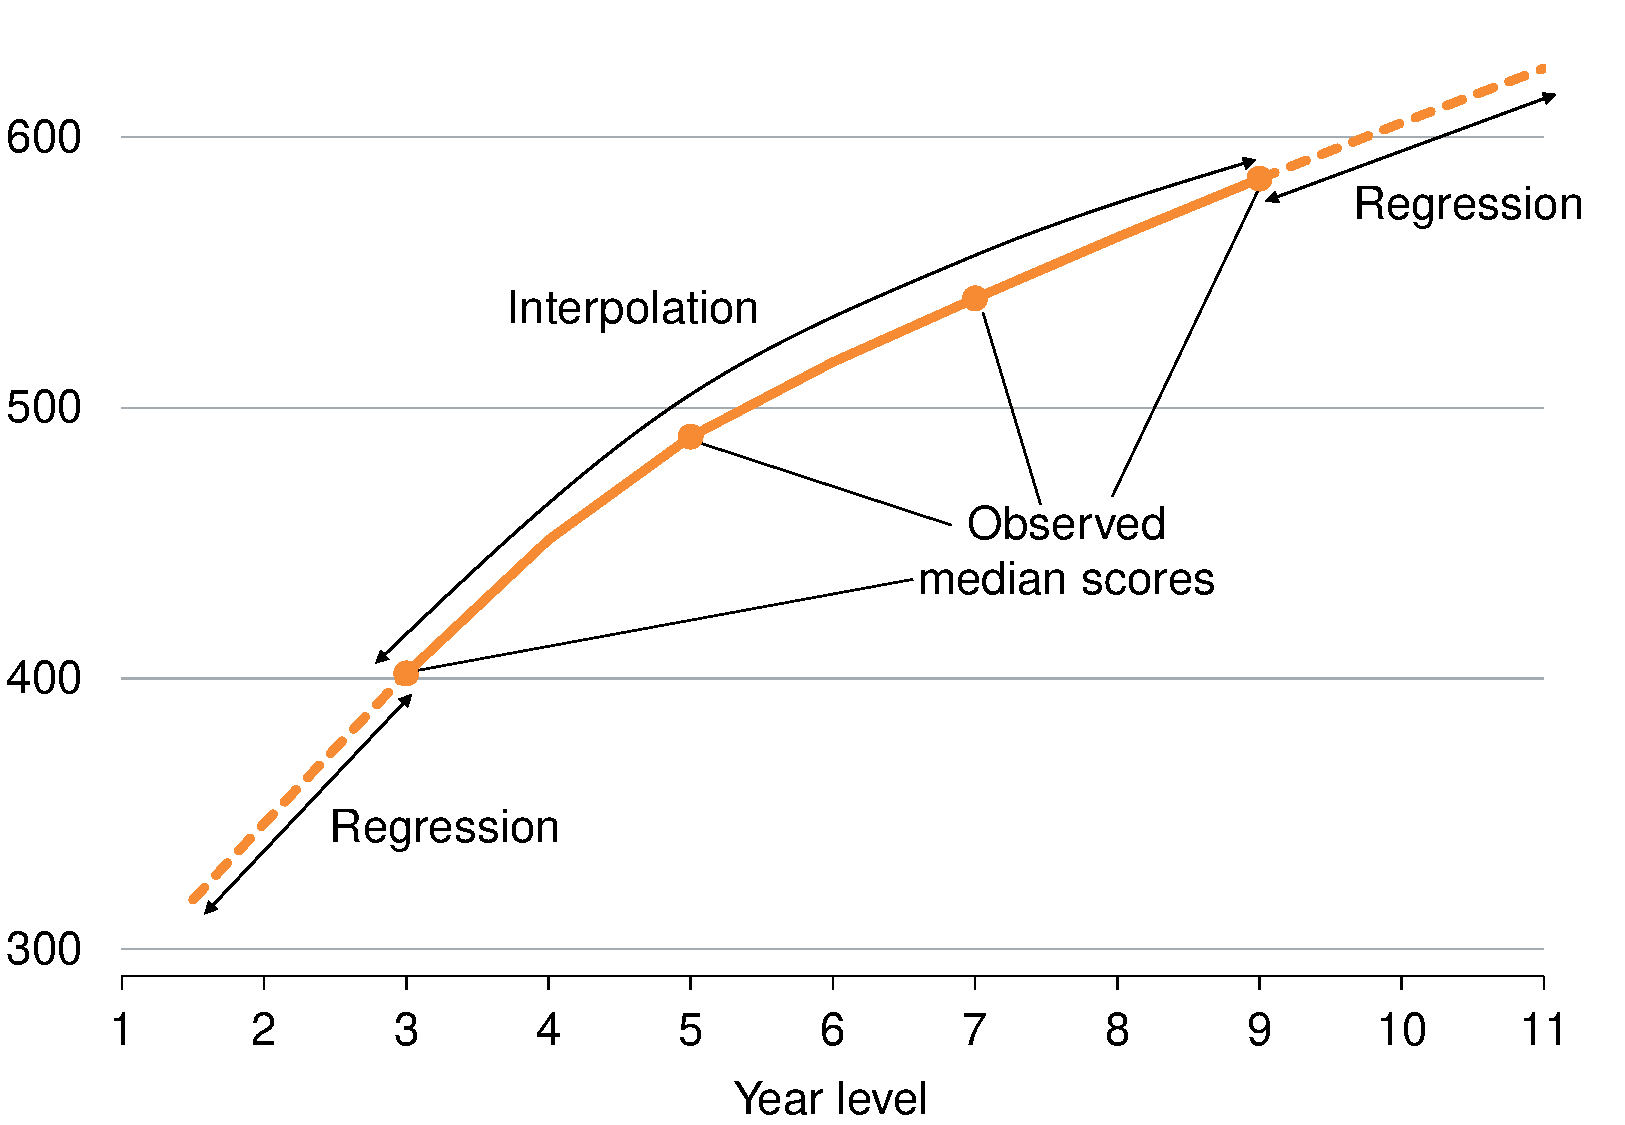
\includegraphics[width=\columnwidth]{atlas/CYL_n.pdf}\label{fig:cyl_n}

\source{Grattan analysis of \textcite{acara2014}.}
\end{figure}

\newpage
Having constructed the benchmark curve, it is possible to track the equivalent years of progress made by a given student or a group of students. An example of this is shown in \Cref{fig:benchmark} for the median student (Student A) of an above-average student group. In \mbox{Year 3}, this student is about one year and seven months ahead of the benchmark curve in \mbox{Year 3}. By tracking Student A back to the benchmark curve, we can conclude that this group made above-average progress between each NAPLAN test, finishing \mbox{Year 9} two years and four months ahead of the benchmark. That is, this student made six years and nine months of progress between \mbox{Year 3} and \mbox{Year 9}.

\newpage
\begin{figure}[H]
 \captionwithunits{Student progress is measured with reference to the benchmark curve}{NAPLAN scale score, numeracy, Australia}
 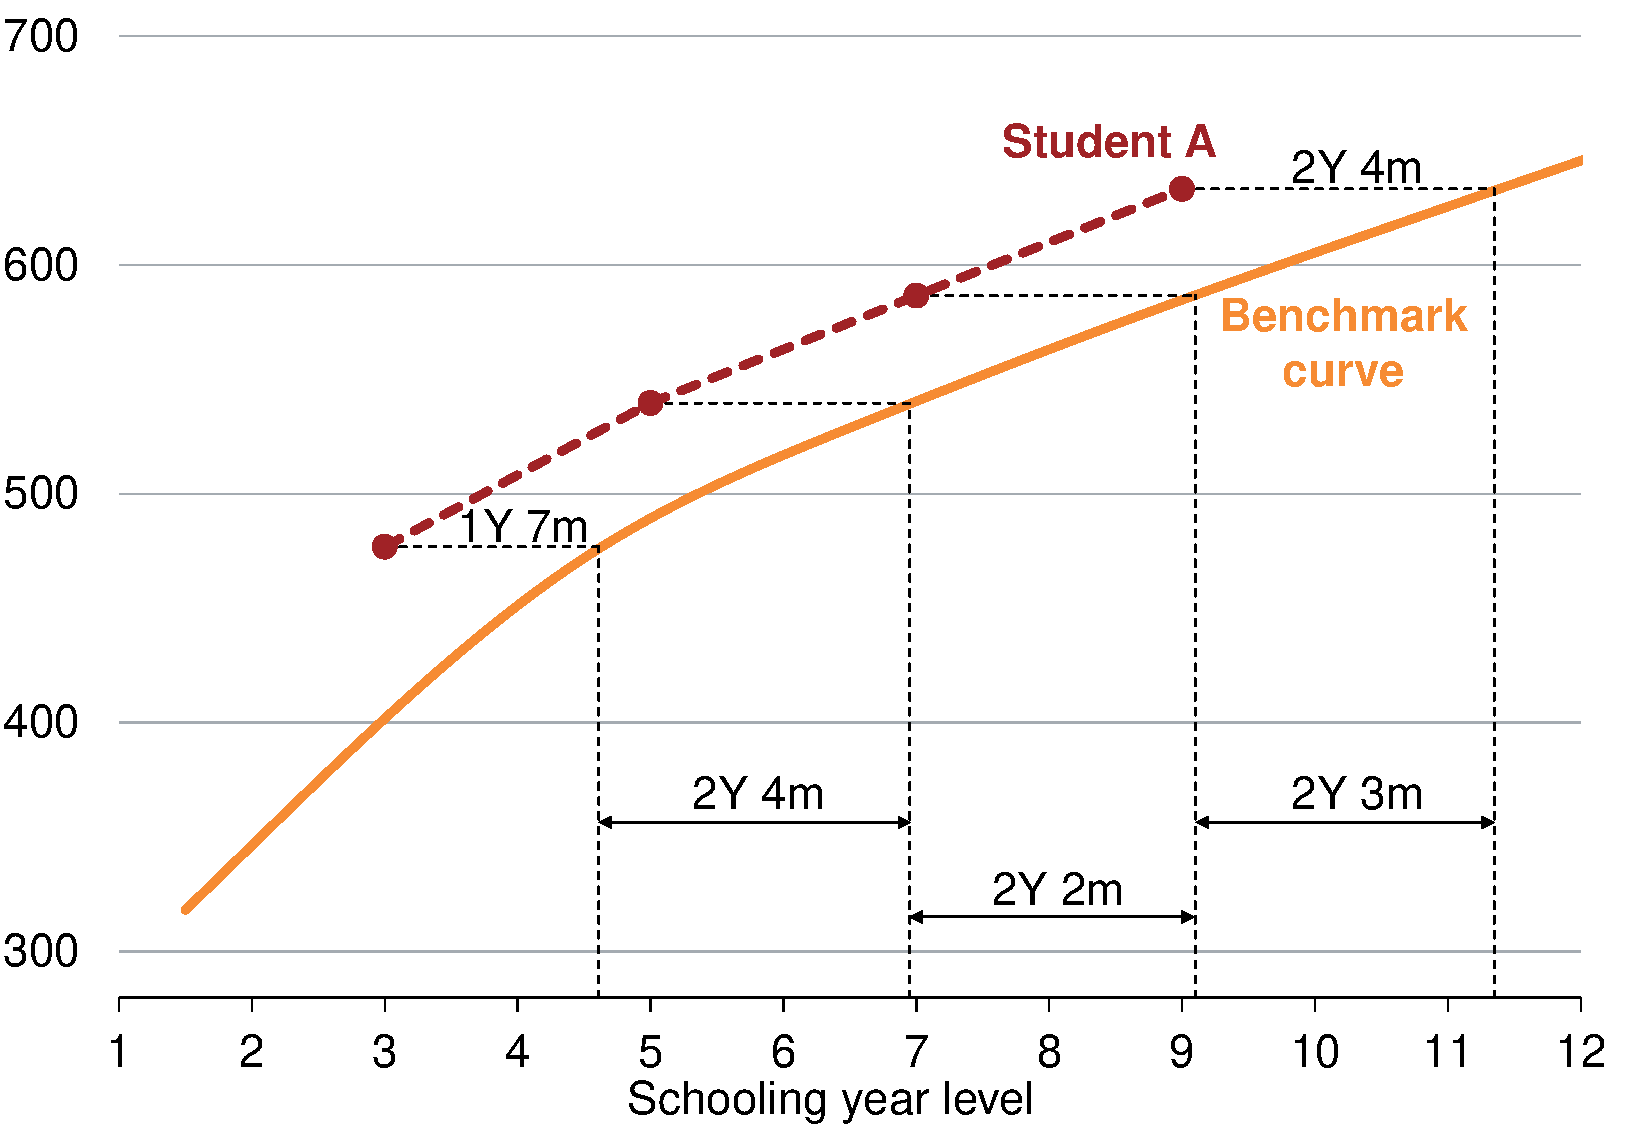
\includegraphics[width=\columnwidth]{atlas/Benchmark_curve.pdf}\label{fig:benchmark}

\source{Grattan analysis of \textcite{acara2014}.}
\end{figure}


\clearpage

\begin{bigparbox*}{How to interpret equivalent year levels}{box:eyl}
\raggedright

Equivalent year levels are a meaningful way of comparing the relative progress made by different sub-groups of students. Measuring progress in years also has an intuitive interpretation not available from NAPLAN gain scores.

Yet equivalent year levels should not be over-interpreted. For instance, some \mbox{Year 5} students are performing at equivalent year level 9 in numeracy -- this does not mean these students would necessarily perform comfortably in mathematics at a \mbox{Year 9} level. In fact, given that these students have not typically been taught the standard mathematics content between Years 6 and 8, we might expect them to struggle with \mbox{Year 9} content.

A better interpretation is to say that students at equivalent year level 9 have a skill level that is about four years ahead of the typical \mbox{Year 5} student. That is, the typical \mbox{Year 5} student is expected to take about four years to reach the skill level of these students at equivalent year level 9. It may be more statistically pure to construct a separate curve for each year level, and interpret all the results relative to that year level (for example, \textit{one year below}, \textit{two years ahead}), but this also adds a layer of complexity to the interpretation of the analysis.

The interpretation of equivalent year levels below 3 requires care. NAPLAN tests are not designed for students below \mbox{Year 3}. While many students in Years 1 and 2 may have comparable reading or numeracy skills to the typical \mbox{Year 3} student, we do not know how well the typical Year 1 or \mbox{Year 2} student would perform on a \mbox{Year 3} NAPLAN test. 

The interpretation of equivalent year levels above 9 is even more challenging. For instance, while we would interpret students at equivalent year level 11 in numeracy to be two years ahead of the typical \mbox{Year 9} student, it is not clear whether the typical \mbox{Year 9} student will reach this skill level in the next two years. This is because subject choices become more specialised (in many states mathematics is not compulsory in \mbox{Year 11}), and it is possible that the skill level of many students will stagnate after \mbox{Year 9}. It may be more correct to say that the typical \mbox{Year 9} student would take two years to reach equivalent year level 11 if they continue to study numeracy in a similar way over the next two years.

Some may argue that without data on students below \mbox{Year 3} and above \mbox{Year 9}, equivalent year levels should not be estimated beyond this range. While there are challenges in estimating and interpreting equivalent year levels outside the \mbox{Year 3} to \mbox{Year 9} range, many sub-groups of students score outside this range. Restricting results to this range would severely limit our understanding of student progress. For instance, each comparison would need a specific benchmark, or otherwise we would only be able to compare relative progress between Years 5 and 7, rather than between Years 3 and 9.\footnote{The broader policy implications and recommendations of \textit{Widening gaps} would be unchanged even with this much narrower interpretation, because the general patterns of student progress that we find between Years 3 and 9 are consistent with what we find between Years 5 and 7.} For policymakers, it is much more useful if student progress can be compared across the majority of schooling years using a single benchmark curve.

\end{bigparbox*}
